\documentclass[12pt,a4paper,openright,twoside]{book}
\usepackage[utf8]{inputenc}
\usepackage{disi-thesis}
\usepackage{code-lstlistings}
\usepackage{notes}
\usepackage{shortcuts}
\usepackage{acronym}

\school{\unibo}
\programme{Corso di Laurea in Ingegneria e Scienze Informatiche}
\title{Eterogeneità dei sistemi di Aggregate Programming: estensione del sistema ScaFi per l'uso di robot Thymio}
\author{Elvis Perlika}
\date{\today}
\subject{Objective Oriented Programming}
\supervisor{Chiar.mo Prof. Mirko Viroli}
\cosupervisor{Dott. Gianluca Aguzzi}
\session{III}
\academicyear{2023-2024}

% Definition of acronyms
\acrodef{IoT}{Internet of Thing}
\acrodef{vm}[VM]{Virtual Machine}
\acrodef{FP}{Functional Programming}
\acrodef{RT}{Referential Transparency}
\acrodef{AP}{Aggregate Programming}

\mainlinespacing{1.241} % line spacing in mainmatter, comment to default (1)

\begin{document}

\frontmatter\frontispiece

\begin{abstract}	
Max 2000 characters, strict.
\end{abstract}

\begin{dedication} % this is optional
    Qualsiasi tecnologia sufficientemente avanzata è indistinguibile dalla magia. \\ Terza Legge di Arthur C. Clarke
\end{dedication}

%----------------------------------------------------------------------------------------
\tableofcontents   
\listoffigures     % (optional) comment if empty
\lstlistoflistings % (optional) comment if empty
%----------------------------------------------------------------------------------------

\mainmatter

%----------------------------------------------------------------------------------------
\chapter{Introduction}
\label{chap:introduction}
%----------------------------------------------------------------------------------------

Write your intro here.
\sidenote{Add sidenotes in this way. They are named after the author of the thesis}

You can use acronyms that your defined previously,
such as \ac{IoT}.
%
If you use acronyms twice,
they will be written in full only once
(indeed, you can mention the \ac{IoT} now without it being fully explained).
%
In some cases, you may need a plural form of the acronym.
%
For instance,
that you are discussing \acp{vm},
you may need both \ac{vm} and \acp{vm}.

\paragraph{Structure of the Thesis}

\note{At the end, describe the structure of the paper}

%----------------------------------------------------------------------------------------
\chapter{Background}
\label{chap:background}
%----------------------------------------------------------------------------------------

I suggest referencing stuff as follows: \cref{fig:random-image} or \Cref{fig:random-image}

% \begin{figure}
%     \centering
%     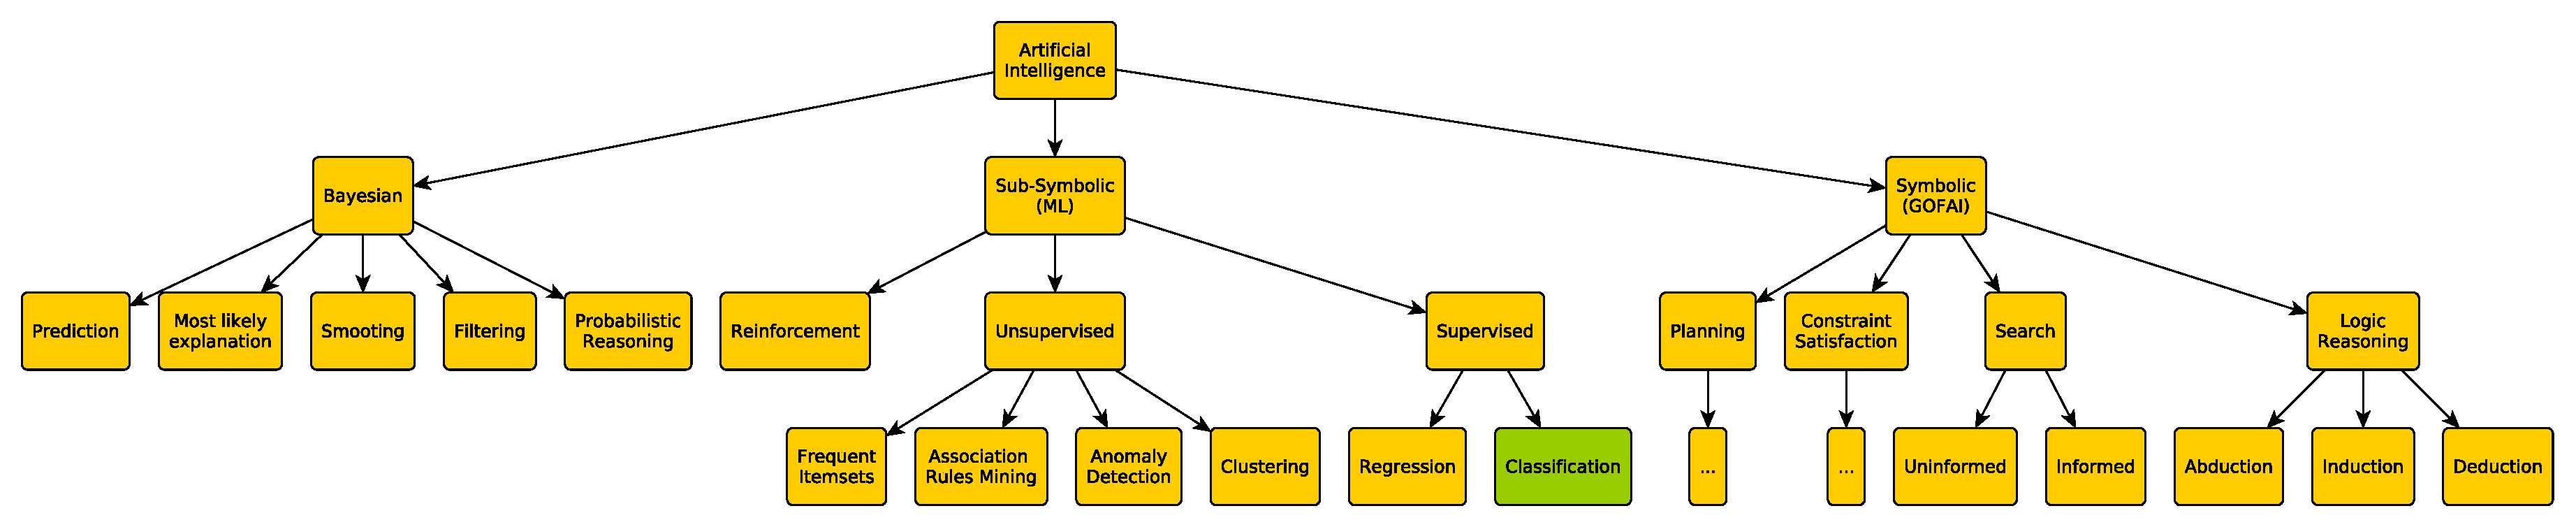
\includegraphics[width=.8\linewidth]{figures/random-image.pdf}
%     \caption{Some random image}
%     \label{fig:random-image}
% \end{figure}

\section{Paradigma OOP e Programmazione Funzionale}

\subsection{Paradigma OOP}

L'Objective Oriented Programming è un paradigma nel senso stretto del termine poichè rappresenta un modo di organizzare e rappresentare un mondo. 
Il paradigma in questione deve la sua potenza nella capacità di simulare entità reali ed è riassumbile con la frase \textit{Everything is an Object}. 
È rilevante parlare di OOP in quanto il paradigma di programmazione funzionale, che è alla base di ScaFi, è un'estensione di esso. 
Il potere della programmazione ad Oggetti (OOP), come detto precedentemente, risiede nella capacità di simulare un mondo e permette di farlo grazie agli "oggetti", essi sono istanze di Classi, le quali a loro volta sono strutture dati astratte che permettono ad ogni loro istanza di avere uno stato (definito dai \textit{fields}) e un comportamento (definito dai \textit{methods}).
I pilastri della programmazione ad oggetti sono l'incapsulamento, l'ereditarietà e il polimorfismo\cref{fig:OOP}.

\begin{figure}
    \centering
    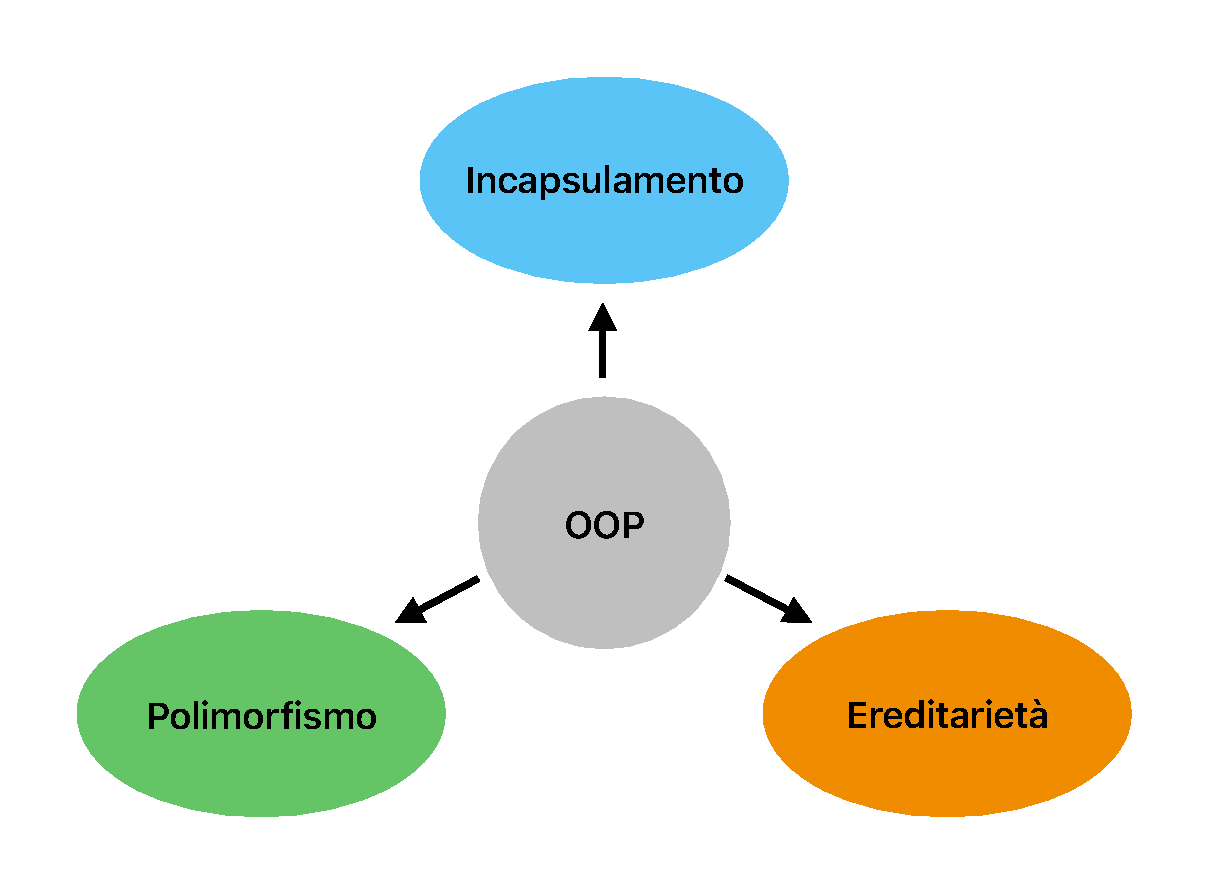
\includegraphics[width=.6\linewidth]{figures/OOP.pdf}
    \caption{Principi della OOP}
    \label{fig:OOP}
\end{figure}

\begin{itemize}
    \item \textbf{Incapsulamento}: Questo principio vuole che i dettagli implementativi di una classe siano nascosti ad altre classi. È un approccio progettuale che mira ad isolare ogni sistema e set di dati. 
    \item \textbf{Ereditarietà}: Con ereditarietà si intende la specializzazione di una classe figlia da una classe madre. Questo permette di creare classi più specifiche che ereditano le proprietà e i metodi della classe madre incoraggiando il riuso del codice.
    \item \textbf{Polimorfismo}: Il polimorfismo è la capacità di un ogetto di assumere più forme. In OOP il polimorfismo è realizzato attraverso l'\textit{overloading} e l'\textit{overriding}. L'overloading è la possibilità di avere più metodi con lo stesso nome ma con diversi parametri \footnote{I parametri possono differire sia in numero che in tipo.}, mentre l'overriding è la possibilità di ridefinire un metodo della classe madre nella classe figlia\footnote{Quando viene chiamato un metodo su un oggetto polimorfico, la scelta di quale implementazione dello stesso metodo scegliere avviene a runtime, in base al tipo effettivo dell'oggetto.}.
\end{itemize}

La programmazione ad oggetti si differenzia dalla più clasica programmazione funzionale in quanto controlla la complessità del software supportando la scomposizione gerarchica attraverso sia i dati che l'astrazione procedurale.
Tra i benefici della OOP troviamo la predisposizione al miglioramento della qualità e della leggibilità del codice e la facilità di manutenzione.

Non è, tuttavia, priva di difetti, richiede un particolare impegno gestire il sistema da realizzzare all'aumentare della sua complessità. Altri paradigmi, come la programmazione funzionale, possono essere più adatti a determinati problemi.

\subsection{Programmazione Funzionale}
Nel caso della OOP abbiamo riassunto il paradigma con la frase \textit{"Everything is an Object"}, per la programmazione funzionale possiamo riassumerla con \textit{"Everything is a Function"}. Quando si parla di funzioni nel ambito della \ac{FP} si intendo \textbf{funzioni pure} cioè senza effetti collaterali. Per effetti collaterali si intende che la fuzione fa altro oltre a restituire un risultato. Un paio di esempi, presi da \texttt{Functional Programming in Scala}, sono:

\begin{itemize}
    \item Modifica di una variabile
    \item Modifica del campo di un oggetto
    \item Leggere da o scrivere su un file
    \item "Disegnare" sullo schermo
\end{itemize}

Si potrebbe pensare che con l'uso della \ac{FP} si possano costruire solo programmi semplice, nella realtà non c'é alcuna limitazione sulla complessità del software da costruire poichè il paradigma della FP esprime un nuovo modo di pensare e scrivere il codice.

Nel dettaglio, per \textbf{funzione pura} si intende una funzione $f:A\to B$, (una funzione che prende un input di tipo $A$ e restituisce un output di tipo $B$) che mette in relazione ogni elemento di $A$ con esattamente un valore di $B$. Qualsiasi altra operazione che non sia utile a calcolare $f(a)=b$ con $a\in A$ e $b\in B$ deve essere intesa come effetto collaterale della funzione e quindi evitata se si vuole creare una funzione pura.

Un esempio di funzione pura, senza effetti collaterali, è la funzione di somma che prende in input due valori e ne restituisce la loro somma. 

\begin{lstlisting}[language=Scala]
    def sum(a: Int, b: Int): Int = a + b
\end{lstlisting}

Formalmente si può definire una funzione pura con il concetto di \ac{RT}:

\begin{quote}
    Una funzione $f$ è Referentially Transparent se per ogni contesto $C$ nel quale la funzione viene inserita, essa può essere sostituta dal risultato della stessa funzione $f$ senza condizionare il risultato di $C$.
\end{quote}

È proprio questa proprietà che permette ad un programma progettato con approccio funzionale di essere maggiormente scalabile e mantenibile.

\section{Paradigma dell'Aggregate Programming}

Nei capitoli precedenti si è esaminata l'evoluzione dal paradigma \ac{OOP} a quello \ac{FP}, la quale, ha pemesso di gestire in modo più pratico progetti più complessi e semplificandone la manutenibilità. Una ulteriore, più specificica, evoluzione è quella portata dal paradigma dell'\ac{AP}. Quest'ultimo mira a rendere la progettazione, manutenzione e testing nell'ambito del controllo di dispositivi hardware di larga-scala.

La tecnica dellì\ac{AP} si basa su 3 principi fondamentali per la costruzione di sistemi robusti e resilienti:

\begin{itemize}
    \item 
\end{itemize}

\section{ScaFi e Macro-Swarm}

\section{Thymio e tdmclient}

\section{Aruco Tag}

%----------------------------------------------------------------------------------------
\chapter{Analisi}
\label{chap:analisi}
%----------------------------------------------------------------------------------------

\section{Estendibilità del sistema ad un nuovo modello di Robot (Thymio)}

\section{Gestione dei vincoli di compatibilità del sistema Thymio}


%----------------------------------------------------------------------------------------
\chapter{Design}
\label{chap:design}
%----------------------------------------------------------------------------------------

\section{Architettura server Flask}

\section{File di configurazione}

%----------------------------------------------------------------------------------------
\chapter{Implementazione}
\label{chap:implementazione}
%----------------------------------------------------------------------------------------

\section{Implementazione del server Flask}

\section{Esempi di Algoritmi AP applicati ai Robot Wave e Thymio nello stesso ambiente}

You may also put some code snippet (which is NOT float by default), eg: \cref{lst:random-code}.

\lstinputlisting[float,language=Java,label={lst:random-code}]{listings/HelloWorld.java}

\section{Fancy formulas here}

%----------------------------------------------------------------------------------------
\chapter{Conclusione}
\label{chap:conclusione}
%----------------------------------------------------------------------------------------

%----------------------------------------------------------------------------------------
% BIBLIOGRAPHY
%----------------------------------------------------------------------------------------

\backmatter

\nocite{*} % Remove this as soon as you have the first citation

\bibliographystyle{alpha}
\bibliography{bibliography}

\begin{acknowledgements} % this is optional
Optional. Max 1 page.
\end{acknowledgements}

\end{document}
